\documentclass[]{article}
\usepackage{xcolor,listings}
\usepackage{textcomp}
\usepackage[margin=1.0 in]{geometry}
\usepackage{graphicx}
\usepackage{biblatex}
\usepackage{hyperref}
\usepackage{subcaption}
\usepackage{amssymb}
\usepackage{lscape}
\usepackage{rotating}
\definecolor{light-gray}{gray}{0.95}
\newcommand{\code}[1]{\colorbox{light-gray}{\texttt{#1}}}
\title{The use of Graph Databases in Genomic Analysis}
\author{Lacey Conrad\\MSDE 692\\ Regis University}
\date{March, 2022}

\begin{document}
	\maketitle
\pagebreak
\vspace{10mm}
{Table of Contents}\\
\\
Section 1: Introduction - 3\\
Section 2: Methods - 3\\
Section 3: Results and Analysis - 4\\
Section 4: Conclusion - 5\\
Section 5: References - 6\\
Section 6: Code - 6\\
Section 7: Figures - 8\\
\pagebreak

\section{Introduction}
Much of the data in the biological sciences is considered complex, often containing many-to-many relationships and the need for frequent data insertions. Genomics data, in particular, represents a multitude of heterogeneous, complex relationships both between variables and data sources. It is data not suited to traditional relational databases, where a query would require numerous join operations, resulting in an inefficient database (Messina et al., 2018; Mughal et al., 2017). 

Graph databases store data in a way where join operations are not needed.  These databases store data records as nodes, and use relationships as pointers to other nodes.  This schema more accurately reflects the relationship of data in genomics, and creates an intuitive design to the database. Even as more relationships and nodes are added to the database, the query time is constant (Huang, S. 2022a; Huang, S. 2022b; Mughal et al., 2017).  

In one example of how a graph database could be used on genomic data, nodes represent genes including their associated functions, and are stored with their relationships to other genes, variants, proteins, pathways, and so on (Huang, S. 2022a; Huang, S. 2022b). The database could even include sparse and irregular relationships between genes, such as when the expression of one gene influences another gene or two genes are expressed together (Mughal et al., 2017). 

While the potential for using graph databases to this end has been noted, graph databases have not been readily accepted by the genomics community despite their intuitive schema, efficient storage and query capabilities. Therefore it makes sense to create an easy-to-use pipeline that provides a pathway between genomic research records and a graph database. Making this technology more accessible to biologists at large would allow them the ability to not only query their data easier, but also utilize graph algorithms that can detect unique relationships within the data (Mughal et al., 2017).

The purpose of this research project was to create a data pipeline that uploads into Neo4J genomic datasets from either a local computer or genomic database. For this first project, a CSV file was downloaded off of the Ensembl website and then modeled into a graph structure after identifying appropriate nodes and vertices. This model was used to create a Neo4J database. New data and relationships were added to determine its feasibility, since new data and relationships are frequently added to genomic data. The final goal of this project was to create a Neo4J database comprised of related genomic data and query it in a manner reflecting typical genomic research needs.






\section{Methods}
**Note: all code is included at the end of this paper, in the "code" section.\\


This project had 3 main stages: data acquisition, data cleaning and conversion into a CSV file, and the creation of the database in Neo4J using Cypher.  I then broke down the stages into the following tasks.

\subsection{Outline of Project}

\begin{enumerate}

\item Part 1 (Weeks 1-2):
During the first phase of this project, the primary goal was to learn about the websites containing genomic databases, what data is stored there, and how to download them.  The data was viewed using Python Pandas, cleaned, and saved as a CSV file. My goals for this phase were:

\begin{itemize}
\item Determine commonly used genomic databases and determine how to retrieve data from them.
\item Understand the data structure of the files obtained from these websites (i.e. dependent and independent variables).
\item Understand how data is obtained from these websites.
\item Download several representative file types to my local machine and explore/clean them in Python.
\item Read-in data file and convert into a data frame.
\item Save processed/cleaned data as a CSV.
\end{itemize}


\item Part 2 (Weeks 3-4):  In part 2 of my project, I examined relationships between variables in the downloaded CSV file.  I also supplied additional relationships and nodes, such as the phylogenetic classification of each species in the graph.  These tasks guided my exploration:

\begin{itemize}
	
\item Determine/describe the relationships between variables in the file. 
\item Decide what the nodes/relationships/properties would be.
\item Determine the initial scale of the database. 
\item Create a graph model similar to what would be created in Neo4J.
\item Consider if there are multiple ways this system can be modeled.
\end{itemize}

The conceptual graph model and Arrows graph model can be viewed in section 7 of this write-up.

\item Part 3 (Weeks 4-6):  This third part introduced me to Neo4j's query language and desktop. I uploaded the CSV file created during the early stages of the project to Neo4j, and each gene was mapped to a node. I added phylogenetic data to illustrate complex, multilevel relationships seen in biological data.  I assigned myself the following tasks:

\begin{itemize}
\item Learn how to upload files and recreate the graph model on Neo4J.
\item Learn Cypher query language through the creation of the database.
\item Upload a simplistic dataset first, possibly following a tutorial.
\item Perform several queries using Cypher.
\item Upload genomic CSV file.
\end{itemize}

\item Part 4 (Week 6):  In part 4, I evaluated my model's adaptability in a real-world scenario.  I focused on what data should be included in each node during my research and whether the relationship was biologically meaningful. My goals were:

\begin{itemize}

\item Determine how well it represents the system.
\item Does my model need to be adjusted?
\item Is important information missing in the model that may change the outcome of the analysis?
\end{itemize}

\item Part 5 (Weeks 4-6):  Finally, I increased my proficiency with Cypher by writing several queries.  Genomic datasets are constantly updated with more accurate predictions of genomes, gene functions, and genetic variants, so I wanted to make sure a biologist could keep up the database to date.  To perform these actions, you must understand how to add, change, and remove nodes and relationships within Neo4J.  The tasks I set for myself were:

\begin{itemize}
\item Investigate adding more data to the database.
\item Learn how to incorporate additional data into the established database
\item Also learn how to add more nodes, relationships, and add or change properties.
\end{itemize}
\end{enumerate}

The overall structure of the project is shown in the flow chart in part 7 of this write-up.








\section{Results and Analysis}
Genomics data exists in numerous file formats, mainly depending on who collected the original data and in what country they collected it. The variability of genomic data and heterogeneity of sources made it difficult to begin this project. Python, and the library BioPython, alleviated some of this burden when loading in many standard file formats. These libraries help parse genomic files and make data frame creation straightforward.


Biologists wrote most historical code to read in, clean, organize, and save genomic data in Python. There is also a number written in other languages, with Perl and R being favorites.  Although these characteristics did not increase the project's difficulty, they illustrate the disparity between approaches to managing genomic data.

\begin{enumerate}
\item Part 1 (Engaging with genomics websites)\\
In my early analyses I focused on learning data acquisition from three websites:

\begin{itemize}	
	\item \url{http://uswest.ensembl.org/index.html}
	\item \url{https://www.ncbi.nlm.nih.gov/genome/}
	\item \url{http://https://genome.ucsc.edu/}
\end{itemize}

Ensembl's BioMart feature allowed me to select specific sets of data to download and gave me options regarding the file format in which I could download it.  As a result, I used Ensembl exclusively for this project.  To keep my Neo4J graph consistent and provide the best chances of observing relationships, I downloaded the first 100 genes on chromosome 3 for humans, chickens, and mice.  The primary purpose of this project was to obtain data and upload it to Neo4J, so I downloaded the files as CSV files.  In the second phase of this project, I hope to handle more file formats.



\item Part 2 (Establishment of relationships between variables)\\
In order to make the database easy to observe and work with, I kept the number of relationships and nodes to a minimum.   Since I already had the data uploaded, I used the relationship between genes and chromosome 3 as my initial relationship.  Finally, I included the phylogenetic classification of the three animals used as models. I was drawn to Neo4J by its ability to create hierarchical organizations and relationships, such as that seen between genes and the phylogeny of the animal.




The Python code used to read-in, clean, and convert the files to CSV can be seen in Appendix A.



\item Part 3 (Upload into Cypher)\\
It was a challenge to upload data to Neo4J initially.  In the Neo4J documentation it is not clearly stated that Neo4J will only read data from a specific input file located within its hierarchy.  Having figured this out, reading in any file became very straightforward.  Additionally, I noticed that the Neo4J server determined the location of the input file, so if I switched servers, I had to make sure to move my data to the new input file.


The relationships were of two types; for chromosome-to-gene, the relationship was "contains," and for the phylogenetic relationships, the label changed to "member of."  I created the gene nodes directly from the downloaded data using Cypher.

The code used to read-in and establish the Neo4J database can be seen in Appendix B.


\item Part 4 (Determine applicability of model)\\
I did not apply graph-specific algorithms when I searched my database; however, it would be beneficial to cluster the genes found in more derived groups of animals to understand the evolution of those genes better.  If the most pertinent data is not included, or if the relationship is misinterpreted, relying on relationships could prove problematic.  It may also be challenging to determine how much data is enough to provide a complete picture of a system.  The question seems then to be: how much data is enough?  Should you include all laboratory results?  I cannot find any clear guidance in the literature.  The best analyses would be achieved by creating a comprehensive model that shows what data you will need before collecting it.  It appears that one needs to look at the big picture of a research question to construct a graph and collect data.  Yet, one of the most common uses of graph databases in genomics research is to examine previously collected data.  I intend to design my graph database schema by determining what question I am trying to answer and what data I need.

\item Part 5 (Further investigate Neo4J)\\
As with the movies tutorial that comes prepackaged with Neo4J, I anticipated needing to upload all my data at once.  Adding new datasets in the same way as the first dataset made adding new datasets to my existing database easy.  Maintaining the same node and relationship labels was essential.  If EN0456 is used as a gene ID for chickens, but EN-0456 is used for humans, these two genes are considered different.  This will yield incorrect query results if we search for genes shared by three species since the query will only return two out of the three expected.  Neo4J includes a favorite script tab to save some of the more complex scripts I have written.  This has saved me a lot of time.
\end{enumerate}

\section{Conclusion}
Despite its 15 year history, Neo4J lacks many online learning resources many other comparably aged databases and programming languages have.  For example, it took me a long time to realize that I needed to have my data in a specific directory; the Neo4J website did not indicate it in the online documentation.  Tutorials were available, yet they frequently relied on data uploaded from websites, not a local machine.  Once I discovered the location of Neo4J’s import file, the process of setting up the database was easy.  As is the case with establishing any database, it was essential to understand how the author organized the data file, the variable names, and their relationship.  Also, managing the data beforehand in a graph model helped establish the nodes and connections.  When I created my graph model, it was clear that there would be more than one way to organize the nodes and relationships.  This made me realize there were ways to manage the graph that misrepresent the data's relationships.

Despite these shortcomings, data with complex relationships, like genomic data, can be stored and analyzed using graph databases and keeping pertinent biological relationships intact.  A complex query, resulting in many joins, would be required to determine which animals share a specific gene in a relational database.  This query is both simple to write and fast to execute for Neo4J and graph databases in general.

In general, I enjoyed working on this project.  As a result, I am grateful for the opportunity to learn Neo4J and Cypher, and I believe they will be valuable tools for me in the future.  I think the project was successful and shows a small portion of the potential that Neo4J has for biological data. I have wanted to study the use of biological data in data engineering since I enrolled in the Data Science program at Regis, and I am happy I was able to combine two of my academic passions.

Having learned how to use Neo4J through this project, I now have a lot of opportunities going forward.  I intend to develop my skills further by adding more data to my database to represent a biological system more accurately, both for this project and on my own. A fascinating future direction would be expanding this database and adding complexity to it. In addition, there does seem to be some research using other NoSQL databases with genomic data, which I may investigate for the next part of my project.

\section{References}


\begin{itemize}
	
	\item Huang, S. 2022a. Analyzing genomes in a graph database. Medium. \url{https://medium.com/geekculture/analyzing-genomes-in-a-graph-database-27a45faa0ae8}
	
	\item Huang, S. 2022b. Turn Neo4j into a genome browser. Medium. \url{https://medium.com/codex/turn-neo4j-into-a-genome-browser-e94c7311dfab}
	
	\item Messina, A., Fiannaca, A., La Paglia, L. et al. 2018. BioGraph: a web application and a graph database for querying and analyzing bioinformatics resources. BMC Syst Biol 12, 98 (2018). https://doi.org/10.1186/s12918-018-0616-4
	
	\item Mughal S, Moghul I, Yu J; UKIRDC, Clark T, Gregory DS, Pontikos N. 2017. Pheno4J: a gene to phenotype graph database. Bioinformatics. 2017 Oct 15;33(20):3317-3319. doi: 10.1093/bioinformatics/btx397. PMID: 28633344.
	
\end{itemize}

\section{Code}

\subsection{Appendix A - Python Code}

\begin{lstlisting}[
	backgroundcolor = \color{lightgray},
	language = Python,
	showspaces = false,
	showstringspaces = false,
	basicstyle = \small\ttfamily,
	numbers = left,
	numberstyle = \tiny,
	commentstyle = \color{gray}
	]
# loading the appropriate libraries
from Bio.SeqIO import parse 
from Bio.SeqRecord import SeqRecord 
from Bio.Seq import Seq 
from Bio import SeqIO
import pylab
import pandas as pd
import numpy as np
import json
import csv 

# reading in the files produced from the BioMart application on the Ensembl website.
# These files were stored locally.
df_mouse = pd.read_csv ('mouse3.txt')
df_human = pd.read_csv ('human3.txt')
df_chicken = pd.read_csv ('chicken3.txt')

# renaming the variables 
df_mouse = df_mouse.rename(columns={'Gene stable ID': 'gene_id', 
	'Transcript stable ID':'transcript_id','Gene start (bp)':
	'gene_start','Gene end (bp)':'gene_end'})

df_human = df_human.rename(columns={'Gene stable ID': 'gene_id', 
	'Transcript stable ID':'transcript_id','Gene start (bp)':
	'gene_start','Gene end (bp)':'gene_end'})

df_chicken = df_chicken.rename(columns={'Gene stable ID': 'gene_id', 
	'Transcript stable ID':'transcript_id','Gene start (bp)':
	'gene_start','Gene end (bp)':'gene_end'})


# since I am looking to see if the model will work and the quantity of data 
# is not important, I decided to restrict each of the data files to the first
# 100 listed genes for each species.
df_mouse = df_mouse.loc[0:99]
df_human = df_human.loc[0:99]
df_chicken = df_chicken.loc[0:99]

# saving the cleaned and reduced gene files in a CSV file located
# within the Neo4J file hierarchy.  The files needed to
# be located within the inport directory for the specific server
# the database is stored on.
df_mouse.to_csv('C:/Users/Lacey/.Neo4jDesktop/relate-data/
dbmss/dbms-9cfc9c3c-4c56-4fb0-bc35-0d47f153a333/import/mouse3')

df_human.to_csv('C:/Users/Lacey/.Neo4jDesktop/relate-data/
dbmss/dbms-9cfc9c3c-4c56-4fb0-bc35-0d47f153a333/import/human')

df_chicken.to_csv('C:/Users/Lacey/.Neo4jDesktop/relate-data/
dbmss/dbms-9cfc9c3c-4c56-4fb0-bc35-0d47f153a333/import/chicken3')

\end{lstlisting}



\subsection{Appendix B - Cypher Code}

\begin{lstlisting}[
	backgroundcolor = \color{lightgray},
	language = Python,
	showspaces = false,
	showstringspaces = false,
	basicstyle = \small\ttfamily,
	numbers = left,
	numberstyle = \tiny,
	commentstyle = \color{gray}
	]
# loading the CSV files that were previously cleaned 
# in Python into Neo4J.  When each file was read-in,
# I created nodes for each gene id.
LOAD CSV WITH HEADERS FROM 'file:///chicken3' AS line
CREATE (:Gene {name: line.transcript_id})

LOAD CSV WITH HEADERS FROM 'file:///mouse3' AS line
CREATE (:Gene {name: line.transcript_id})

LOAD CSV WITH HEADERS FROM 'file:///human3' AS line
CREATE (:Gene {name: line.transcript_id})

# nodes were created for chromosome 3 for each species:
CREATE (:Chromosome{number: '3-ms'})
CREATE (:Chromosome{number: '3-ch'})
CREATE (:Chromosome{number: '3-hu'})

# nodes were also created for phylogenetic hierarchy:
#(I'm only showing one for brevity)
CREATE (:Family{name: 'Aves'})

# Relationships were created between the chromosome and the
# genes, and then the chromosome and the phylogenetic
# hierarchy.  These relationships could be created using the
# same basic formula as shown below. Once again, I am only
# showing one example.
MATCH (a:Chromosome), (b:Family)
WHERE a.number = '3-ch' AND b.name = 'Aves;
CREATE (a)-[r:CONTAINS]->(b)
RETURN type(r)
\end{lstlisting}


\section{Figures}
\begin{figure}[!h]
	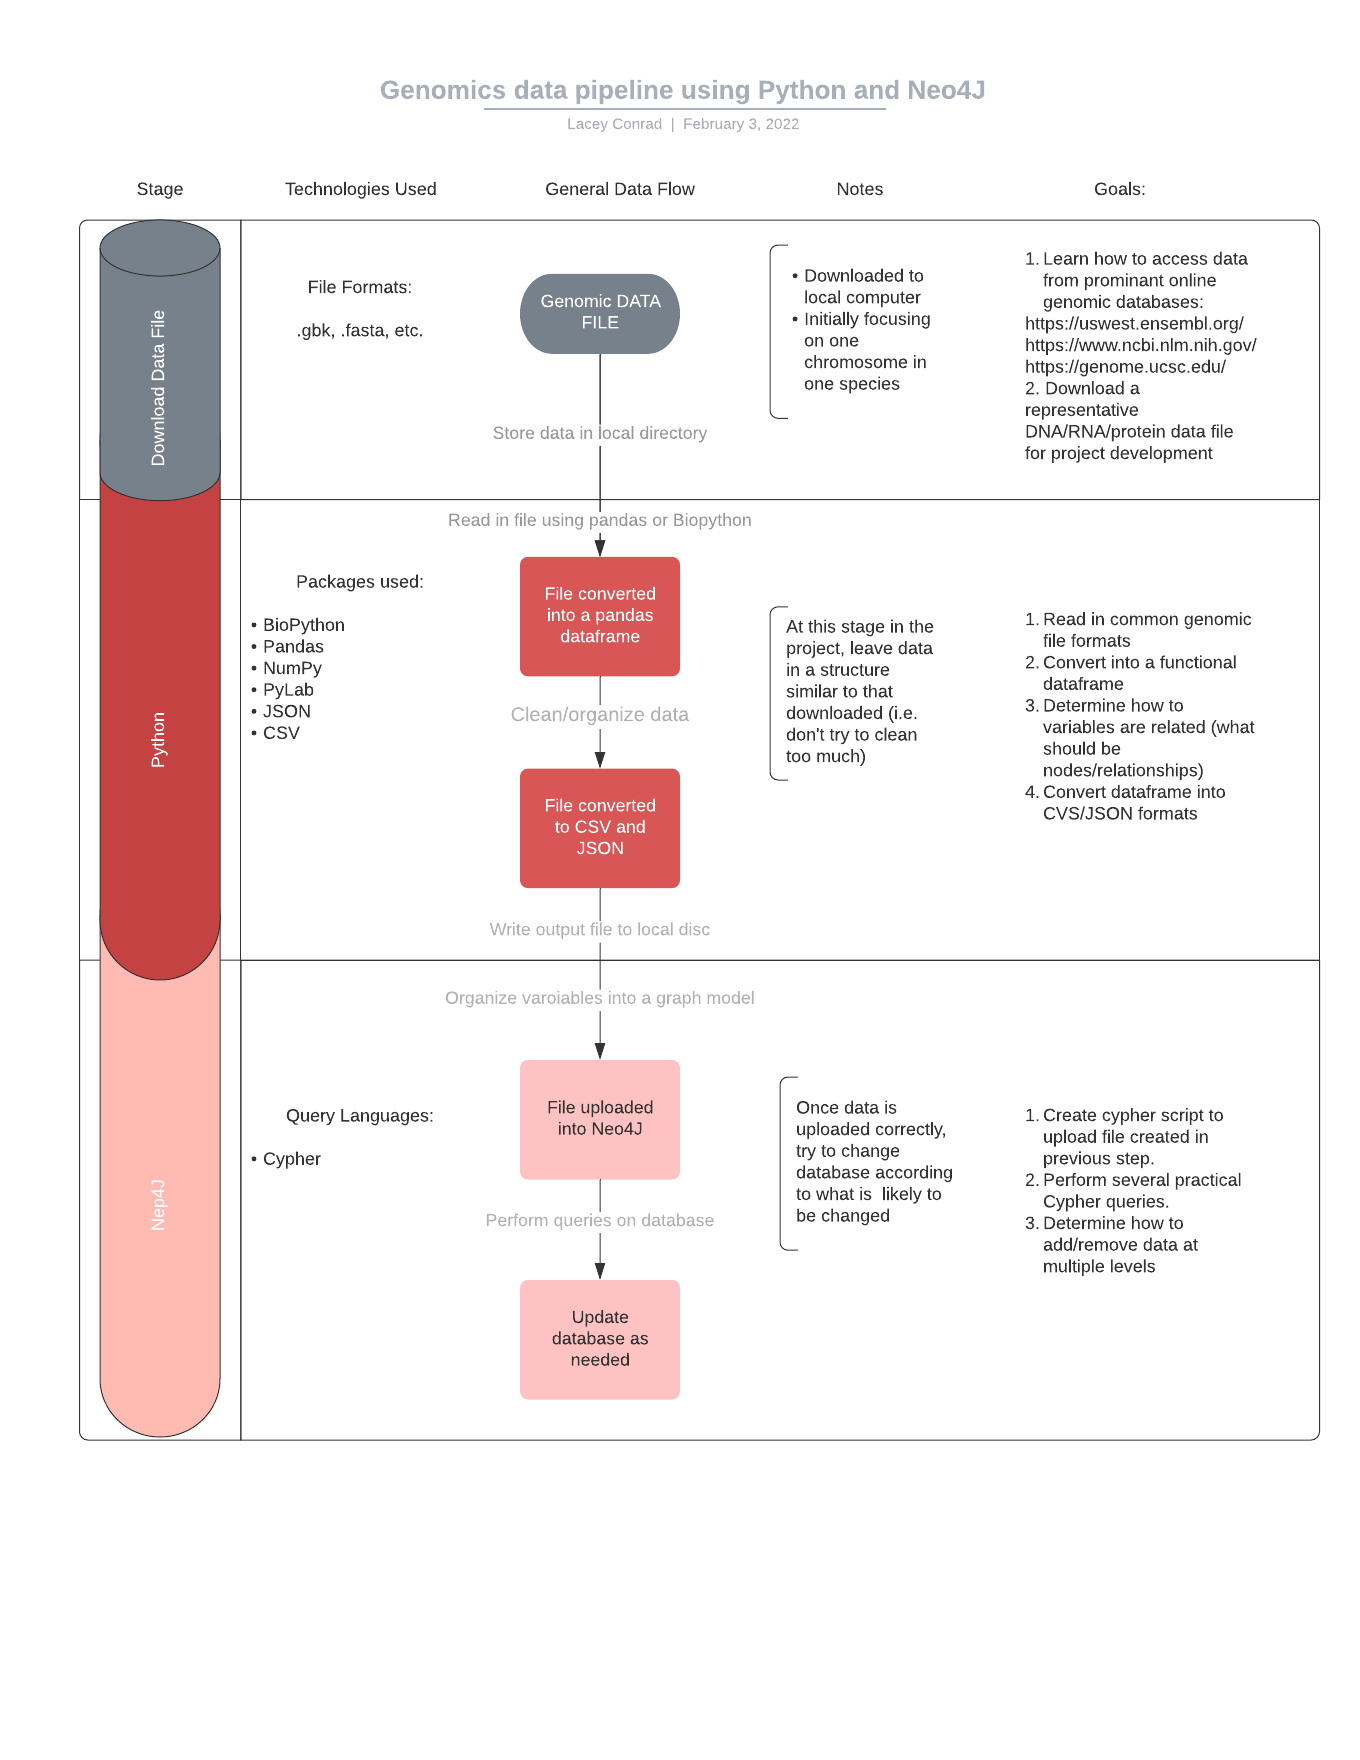
\includegraphics[scale=0.70]{data_pipeline}
	\caption{The overall flow of my genomic graph database project.}
	\label{Fig:Race}
\end{figure}

\begin{figure}[!h]
	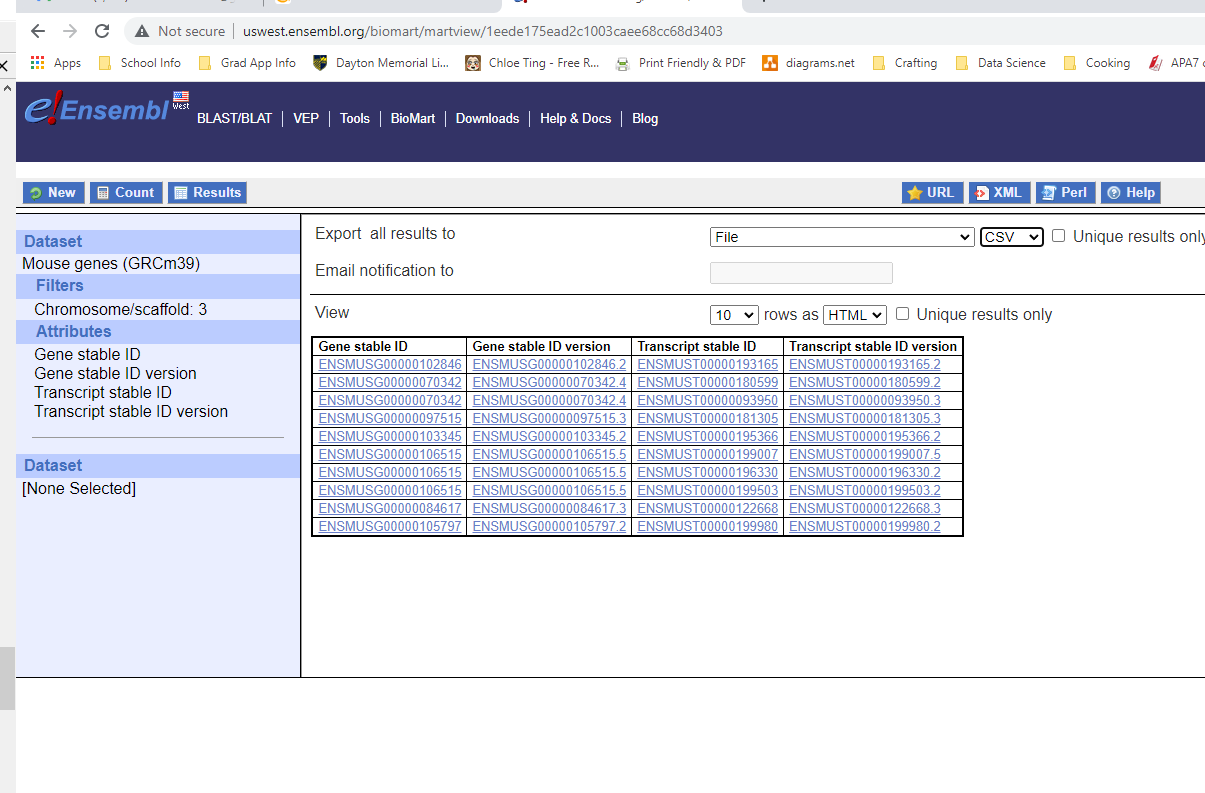
\includegraphics[scale=0.50]{ensemb}
	\caption{The results of a search performed on the BioMart data repository on the Ensembl website.}
	\label{Fig:Race}
\end{figure}





\begin{figure}[!h]
	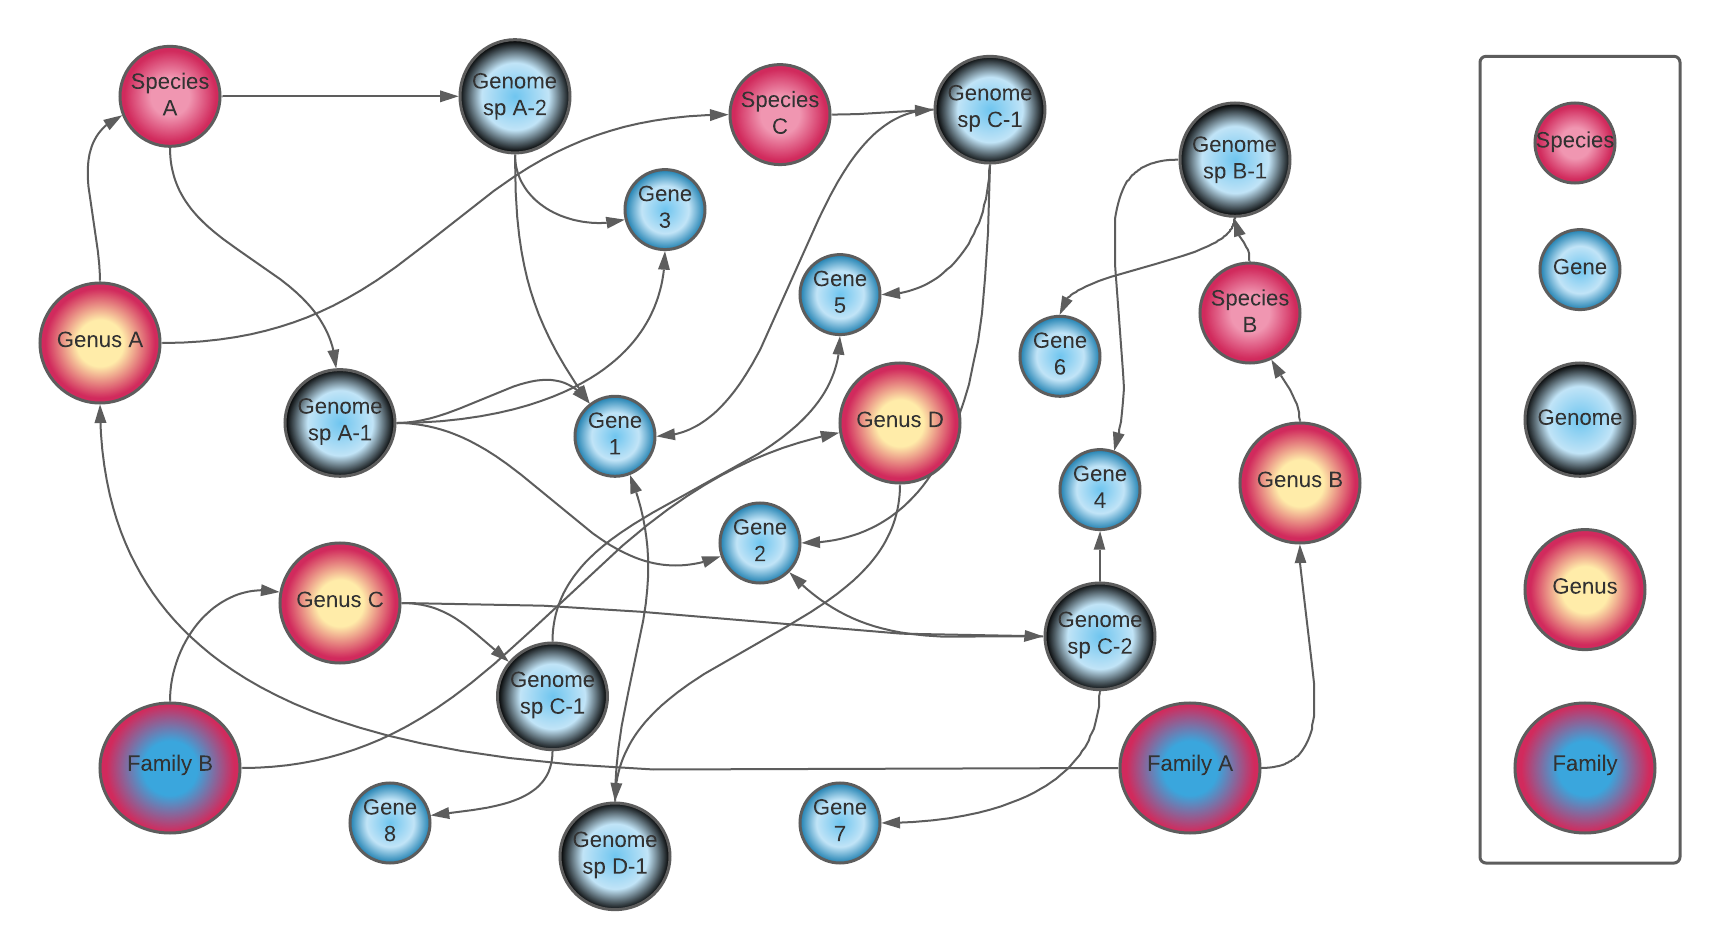
\includegraphics[scale=0.70]{graph model}
	\caption{Conceptual model of the genomic database.}
	\label{Fig:Race}
\end{figure}

\begin{figure}[!h]
	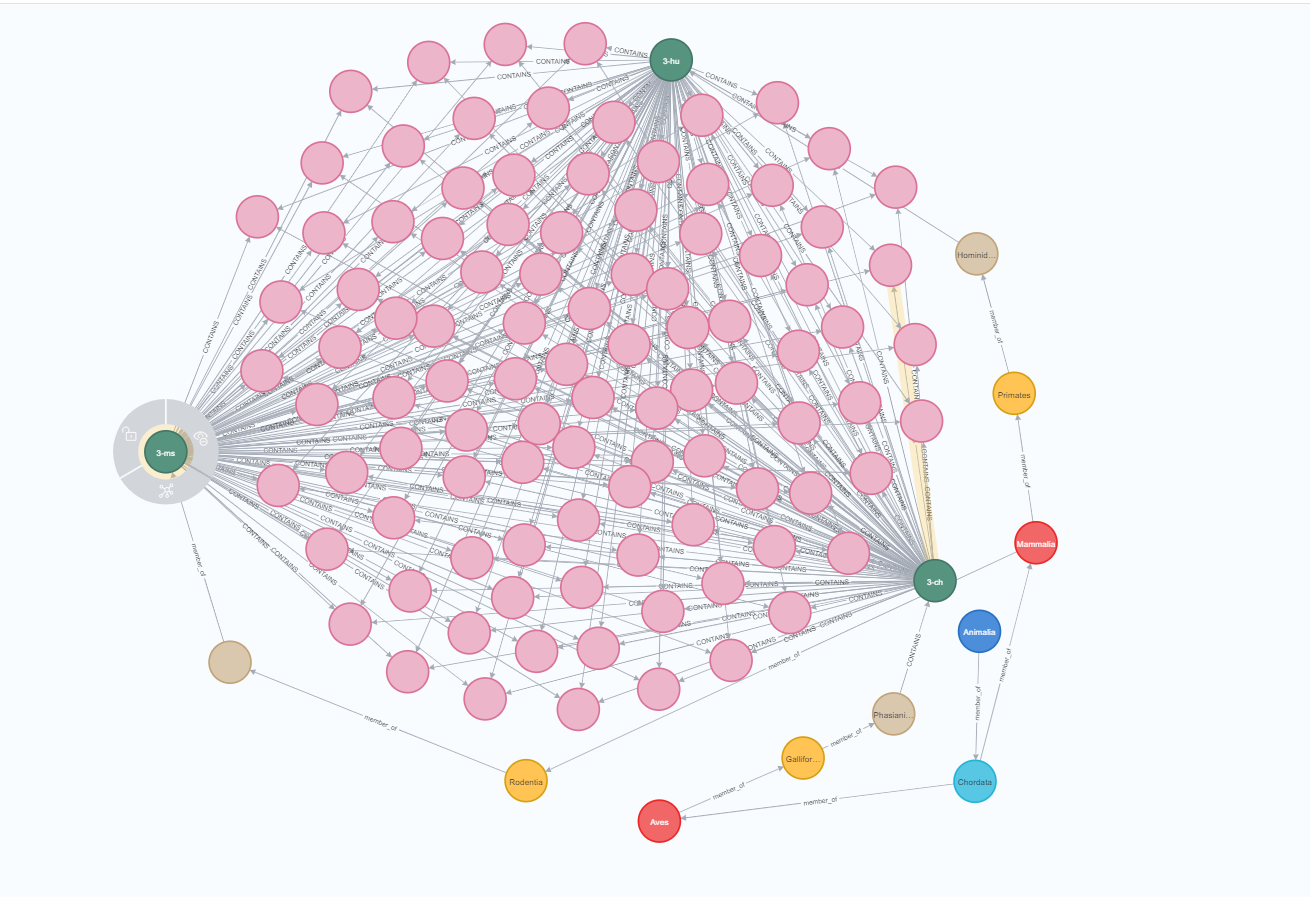
\includegraphics[scale=0.65]{final_db}
	\caption{My complete genomic graph database in Neo4J.  Genes are red; chromosomes are green, and the remaining nodes are phylogenetic hierarchy (Kingdom - Phylum - Class - Order - Family).}
	\label{Fig:Race}
	
\end{figure}

\end{document}